\begin{figure}[htp]
	\centering
	\subfloat[\(\Re\big\{\pixel{S_{1}}\big\},\ \mu=1.00\)] % chktex 21
	{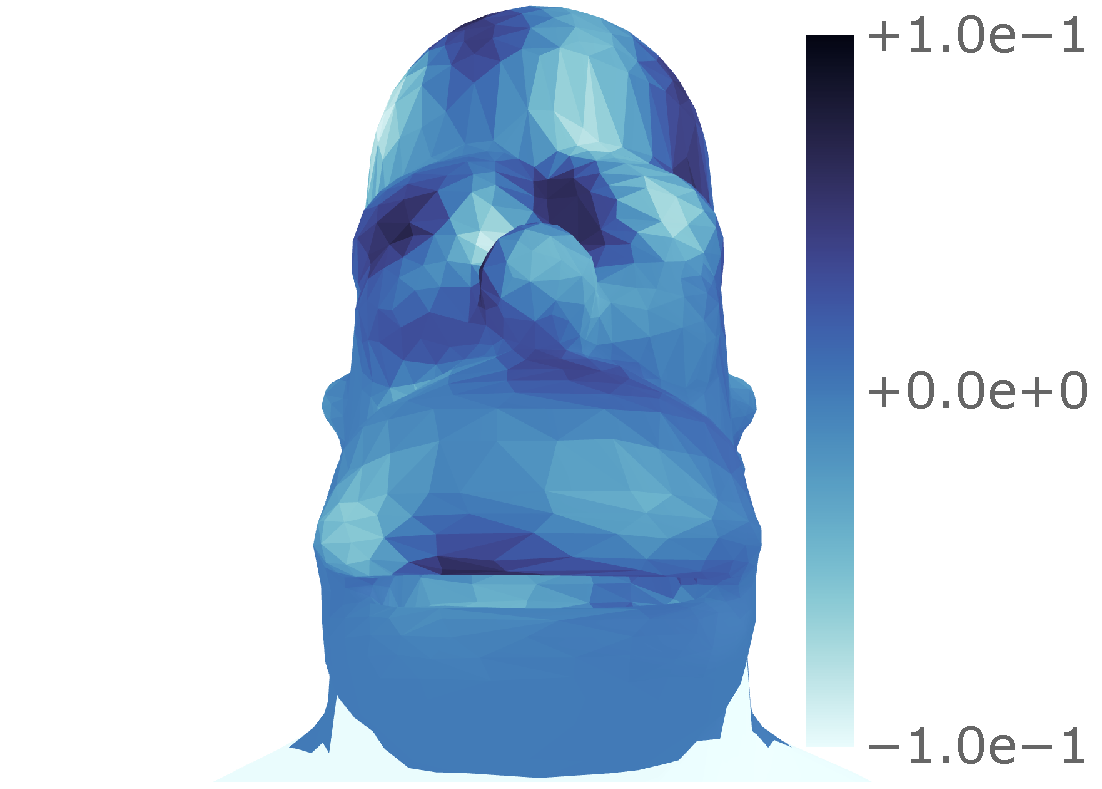
\includegraphics[trim={102 3 6 2},clip,width=.33\textwidth]{slepian_homer_rank0_lam1-000000e00_zoom.pdf}} % chktex 8
	\hfill
	\subfloat[\(\Re\big\{\pixel{S_{10}}\big\},\ \mu=1.00\)] % chktex 21
	{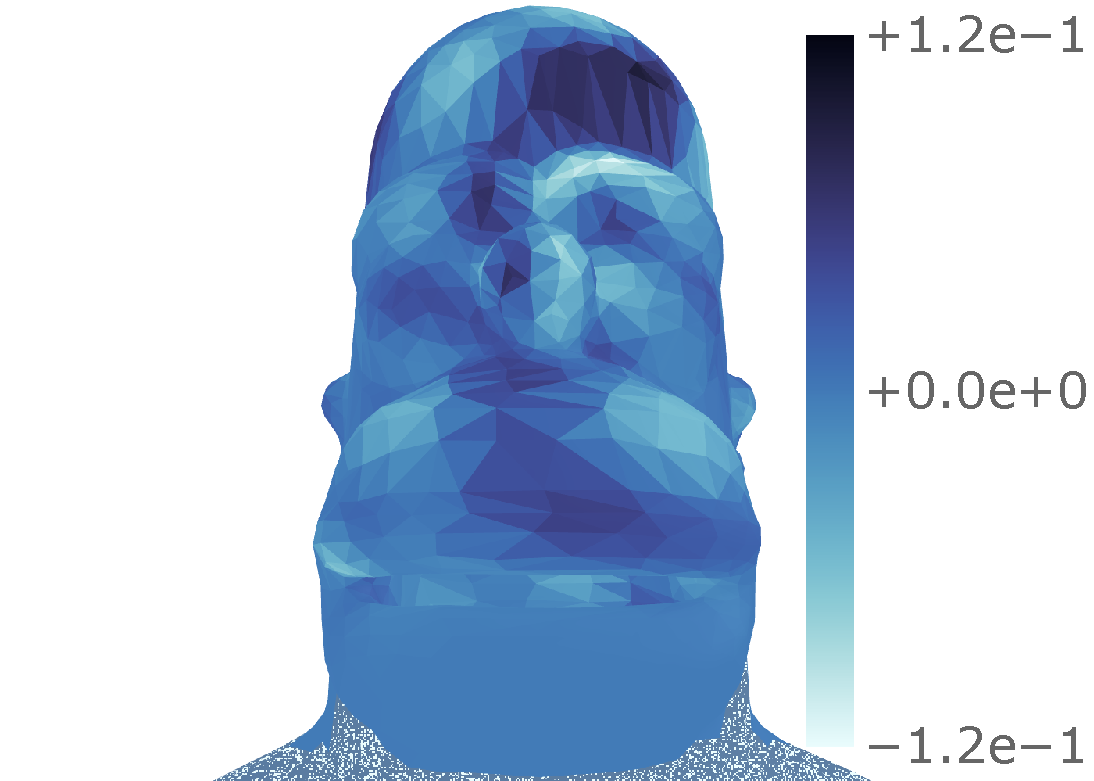
\includegraphics[trim={102 3 6 2},clip,width=.33\textwidth]{slepian_homer_rank9_lam1-000000e00_zoom.pdf}} % chktex 8
	\hfill
	\subfloat[\(\Re\big\{\pixel{S_{25}}\big\},\ \mu=1.00\)] % chktex 21
	{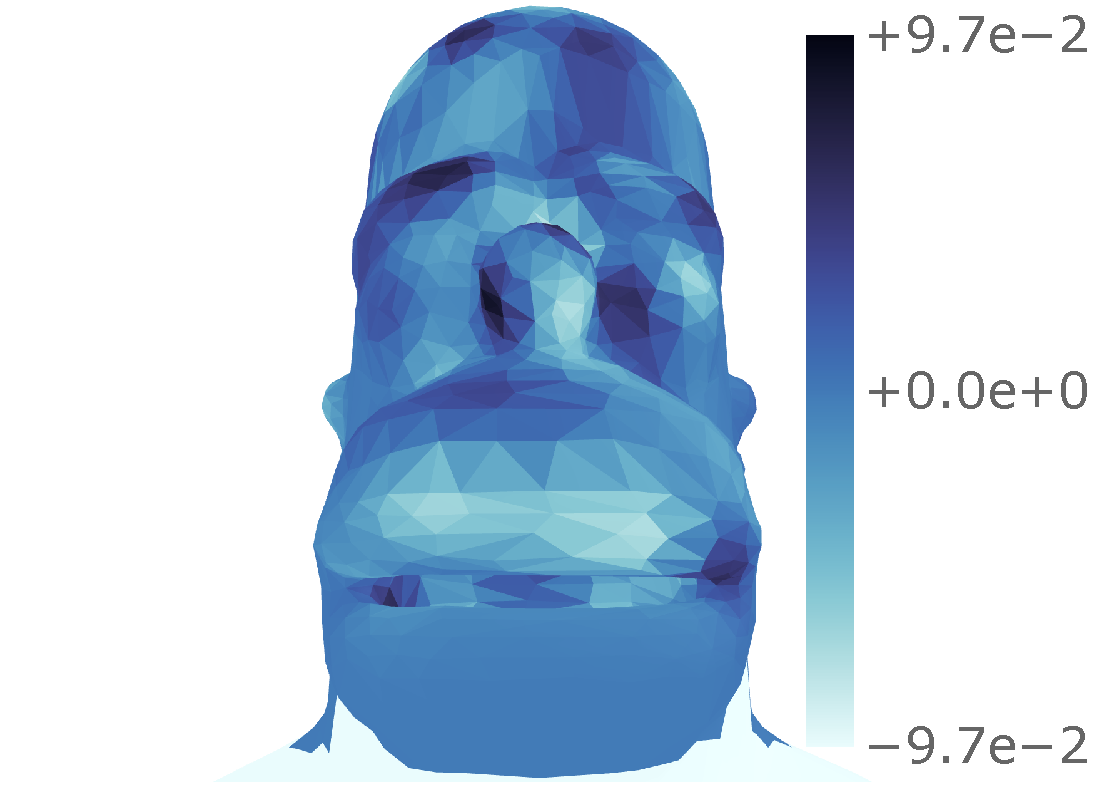
\includegraphics[trim={102 3 6 2},clip,width=.33\textwidth]{slepian_homer_rank24_lam1-000000e00_zoom.pdf}} % chktex 8
	\newline
	\subfloat[\(\Re\big\{\pixel{S_{50}}\big\},\ \mu=1.00\)] % chktex 21
	{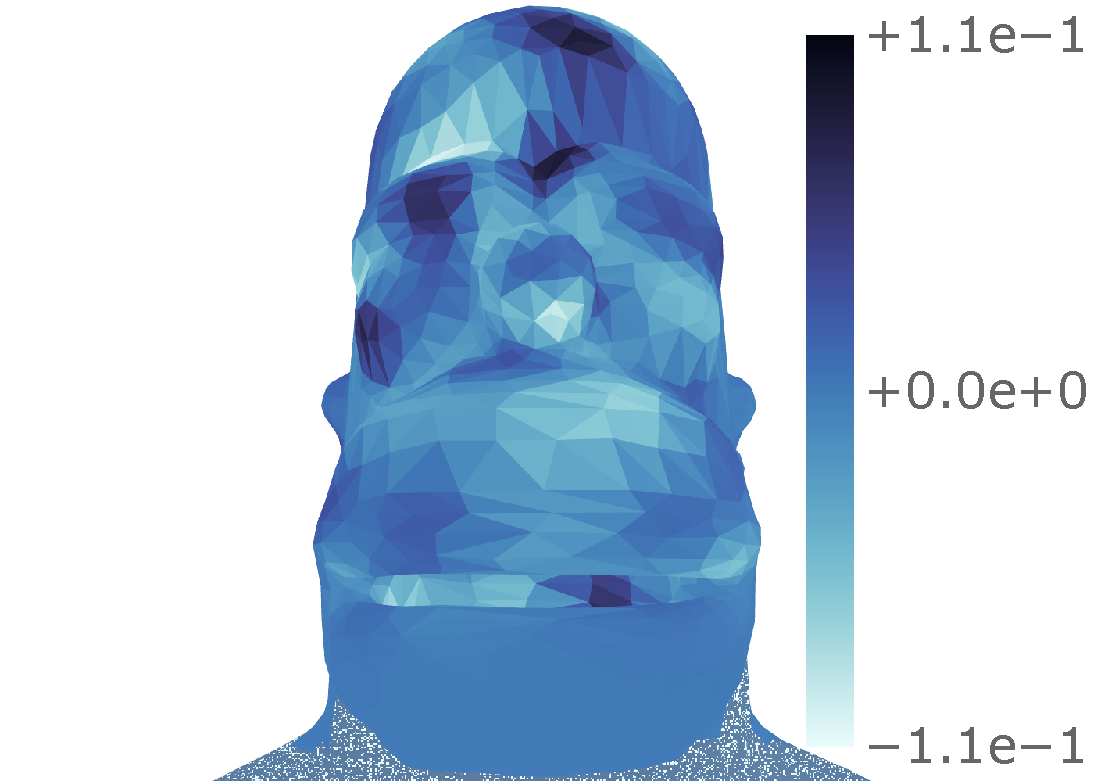
\includegraphics[trim={102 3 6 2},clip,width=.33\textwidth]{slepian_homer_rank49_lam1-000000e00_zoom.pdf}} % chktex 8
	\hfill
	\subfloat[\(\Re\big\{\pixel{S_{100}}\big\},\ \mu=1.00\)] % chktex 21
	{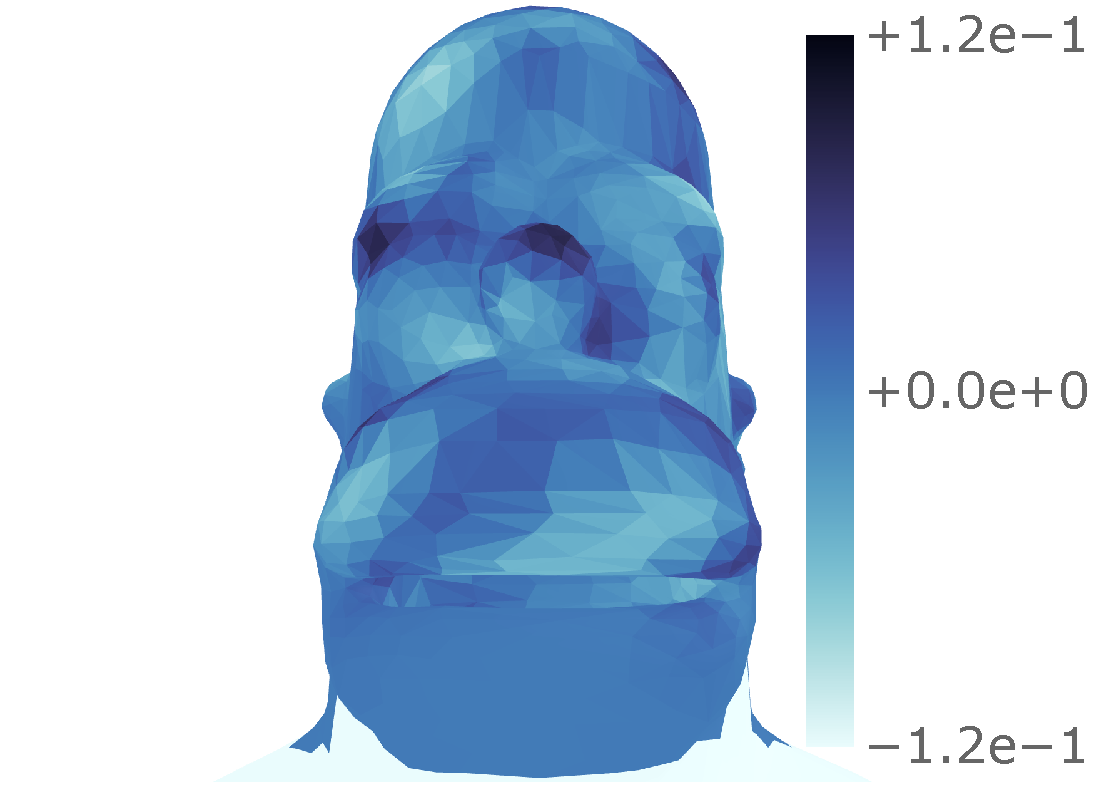
\includegraphics[trim={102 3 6 2},clip,width=.33\textwidth]{slepian_homer_rank99_lam1-000000e00_zoom.pdf}} % chktex 8
	\hfill
	\subfloat[\(\Re\big\{\pixel{S_{200}}\big\},\ \mu=1.00\)] % chktex 21
	{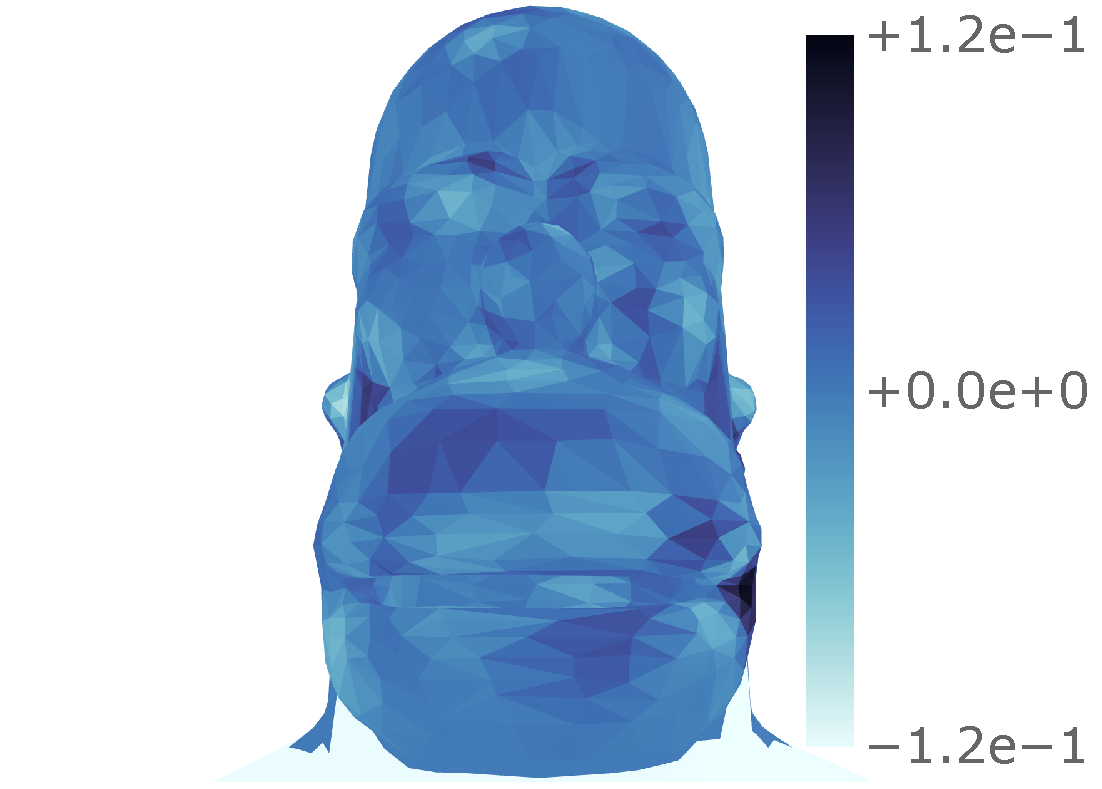
\includegraphics[trim={102 3 6 2},clip,width=.33\textwidth]{slepian_homer_rank199_lam1-000000e00_zoom.pdf}} % chktex 8
	\caption{
	}\label{fig:chapter4_slepian_functions}
\end{figure}
